\documentclass[a5paper,oneside]{amsart}
\usepackage[scale={.9,.9}]{geometry}
\usepackage{mathrsfs}
\theoremstyle{plain}
\newtheorem{theorem}{Theorem}
\newtheorem{lemma}{Lemma}
\newtheorem{corollary}{Corollary}
\newtheorem{proposition}{Proposition}
\newtheorem{conjecture}{Conjecture}
\theoremstyle{definition}
\newtheorem{problema}{Problema}
\newtheorem{ejercicio}{Ejercicio}
\newtheorem*{definition}{Definition}
\newtheorem*{remark}{Remark}
\usepackage{listings}
\usepackage{graphicx}
\lstset{
language=R,
basicstyle=%\scriptsize
\ttfamily,
commentstyle=\ttfamily\color{gray},
numbers=none,
numberstyle=\ttfamily\color{gray}\footnotesize,
stepnumber=1,
numbersep=5pt,
backgroundcolor=\color{white},
showspaces=false,
showstringspaces=false,
showtabs=false,
frame=none,
tabsize=4,
captionpos=b,
breaklines=true,
breakatwhitespace=false,
title=\lstname,
escapeinside={},
keywordstyle={},
morekeywords={}
}
\title[Problemas de Procesos I]{Problemas Resueltos de Procesos Estoc\'asticos I\\ Semestre 2013-II\\ Posgrado en Ciencias Matem\'aticas\\ Universidad Nacional Aut\'onoma de M\'exico}
\author{Jos\'e Adri\'an Ord\'oñez G\'omez}
%\address{}
\usepackage[colorlinks,citecolor=blue,urlcolor=blue]{hyperref}
%\setlength{\textwidth}{17.2cm} % was 18.2
%\setlength{\textheight}{23cm} % was 23
%\setlength{\torgin}{-1cm} % was 0
%\setlength{\oddsidemargin}{-0.6cm}
%\setlength{\evensidemargin}{-0.6cm}

%\setlength{\textwidth}{18.9cm} % was 18.2
%\setlength{\textheight}{26.73cm} % was 23
%\setlength{\topmargin}{1cm} % was 0
%\setlength{\oddsidemargin}{0cm} %
%\setlength{\evensidemargin}{.8cm}
%% Arreglar pues ahora utilizas papel A4.

%Operadores

\DeclareMathOperator{\ivp}{IVP} %
\DeclareMathOperator{\sgn}{sgn} %
\DeclareMathOperator{\md}{mod}
\DeclareMathOperator{\ima}{Im}%
\DeclareMathOperator{\id}{Id} %
\DeclareMathOperator{\homo}{Hom} %
\DeclareMathOperator{\inter}{Int}
\DeclareMathOperator*{\Lim}{lim}
\DeclareMathOperator*{\Limsup}{lim\ sup}
\DeclareMathOperator*{\Liminf}{lim\ inf}
\DeclareMathOperator*{\Min}{m\text{\ii}n}
\DeclareMathOperator{\Aff}{Aff}
\DeclareMathOperator{\Affb}{\overline{\Aff}}
\DeclareMathOperator{\sdfd}{dfd}
\DeclareMathOperator{\scdfd}{dfd}
\DeclareMathOperator{\Beta}{B}
\DeclareMathOperator{\pd}{PD}
\DeclareMathOperator{\supp}{supp}
\DeclareMathOperator{\diam}{diam}
\newcommand{\ind}{\operatornamewithlimits{\perp}}
\DeclareMathOperator{\av}{Abs}
\DeclareMathOperator{\cb}{CB}
\DeclareMathOperator{\cbi}{CBI}
\DeclareMathOperator{\gwi}{GWI}
\DeclareMathOperator{\gw}{GW}
\newcommand{\rtree}{$\re$\nbd tree}
\newcommand{\leb}{\text{Leb}}
%Notaci�n



%Delimitadores
\newcommand{\ceil}[1]{\ensuremath{\lceil #1 \rceil}}
%\renewcommand{\floor}[1]{\ensuremath{\lfloor #1 \rfloor}}

%Formato
\newcommand{\defin}[1]{{\bf #1}}
\newcommand{\mc}[1]{\ensuremath{\mathscr{#1}}}
\newcommand{\bb}[1]{\mathbb{#1}}


%Notation

\newcommand{\card}[1]{\ensuremath{\left| #1 \right|}}
\newcommand{\lccb}{LCCB}
\newcommand{\pss}{S}
\newcommand{\compact}{K}
\newcommand{\psm}{\rho}
\newcommand{\ps}{\paren{\pss,\psm}}
\newcommand{\pse}{x}
\newcommand{\psep}{y}
\newcommand{\psepp}{z}
\newcommand{\saps}{\B_{\pss}}
\newcommand{\bre}{\B_{\re}}
\newcommand{\sko}{D}
\newcommand{\trees}{T}
\newcommand{\C}{C}
\newcommand{\refm}{\mu}
\newcommand{\den}{p}
\newcommand{\psd}[1]{\mc{P}_{#1}}
\newcommand{\s}{\ensuremath{\sigma}}
\newcommand{\bden}{M}
\newcommand{\hh}[1]{{\bf H#1}}
\newcommand{\ball}[2]{\imf{B_{#1}}{#2}}
\newcommand{\mmc}[1]{\imf{\tilde\omega}{#1}}
\newcommand{\rg}[1]{\ensuremath{\imf{\mathbb{G}}{#1}}}




\newcommand{\dfd}{\ensuremath{\stackrel{\sdfd}{=}}}
\newcommand{\deq}{\ensuremath{\stackrel{d}{=}}}

\newcommand{\ley}[2]{\ensuremath{\imf{\mc{L}^{#2}}{#1}}}
\newcommand{\leyc}[3]{\ensuremath{\imf{\mc{L}^{#3}}{#1\left|#2\right.}}}
\newcommand{\cond}[2]{\left.\vphantom{#2}#1\ \right| #2}

\newcommand{\e}{\ensuremath{\mathbf{e}}}
\newcommand{\esf}{\ensuremath{\mc{S}^{\downarrow}}}
%\newcommand{\ps}[1]{\mathscr{P}\paren{#1}}
\newcommand{\fun}[3]{\ensuremath{#1:#2\to #3}}
\newcommand{\fund}[3]{\ensuremath{#1:#2\mapsto #3}}
\newcommand{\set}[1]{\ensuremath{\left\{ #1\right\} }}
\newcommand{\sets}[1]{\ensuremath{{\mathbf #1}}}
\newcommand{\paren}[1]{\ensuremath{\left( #1\right) }}
\newcommand{\bra}[1]{\ensuremath{\left[ #1\right] }}
\newcommand{\seq}[1]{\ensuremath{ #1 _1,\ldots ,#1 _n }}
\newcommand{\sm}[3]{\left[ #1\right]_{#2}^{#3}}
\newcommand{\cde}{\Rightarrow}
\newcommand{\cdfd}{\ensuremath{\stackrel{\scdfd}{\cde}}}
\newcommand{\convo}[2]{\ensuremath{#2^{\!* #1}}}

\newcommand{\tl}[1]{\ensuremath{\hat{#1}}}

\newcommand{\matt}[3]{#1_{#2\, #3}}
\newcommand{\sip}{\bb{P}}
\newcommand{\jump}[2]{\ensuremath{\Delta #1_{#2}}}
\newcommand{\cadlag}{c\`adl\`ag}
\newcommand{\se}{\ensuremath{\bb{E}}}
\newcommand{\ssa}{\ensuremath{\mathscr{F}}}
\newcommand{\si}{{\ensuremath{\bf{1}}}}
\newcommand{\sbr}{\ensuremath{\mc{B}_{\re}}}
%\newcommand{\siind}{\ensuremath{\perp}}
\newcommand{\sigam}{\ensuremath{\Gamma}}
\newcommand{\smc}{\ensuremath{m}}
\newcommand{\sfleche}{S^{\downarrow}_f}

\newcommand{\gafun}[1]{\sigam \paren{#1}}
\newcommand{\poi}[1]{\ensuremath{\mc{P}\!_{#1}}}
\newcommand{\ber}[1]{\ensuremath{\mc{B}\!_{#1}}}
\newcommand{\fcpoi}[1]{\ensuremath{\hat{\mc{P}}\!_{#1}}}
%\newcommand{\ind}{\siind}
\newcommand{\condind}[3]{\ensuremath{#1\ind_{#3}#2}}
\newcommand{\sig}[1]{$\sigma$-\nobreakdash #1}
\newcommand{\sa}{\ensuremath{\sigma}\nbd field}
\newcommand{\realtree}{\ensuremath{\re}\nbd tree}
\newcommand{\eps}{\ensuremath{ \varepsilon}}
\newcommand{\na}{\ensuremath{\mathbb{N}}}
\newcommand{\en}{\ensuremath{\mathbb{Z}_+}}
\newcommand{\eti}{\ensuremath{\mc{U}}}
\newcommand{\etic}{\ensuremath{\mathbb{U}}}
\newcommand{\z}{\ensuremath{\mathbb{Z}}}
\newcommand{\re}{\ensuremath{\mathbb{R}}}
\newcommand{\ra}{\ensuremath{\mathbb{Q}}}
\newcommand{\com}{\ensuremath{\mathbb{C}}}
\newcommand{\con}[1]{\ensuremath{\overline{#1}}}
\newcommand{\proba}[1]{\ensuremath{\sip\! \left( #1 \right)}}
\newcommand{\probas}[2]{\ensuremath{#1\! \left( #2 \right)}}
\newcommand{\probac}[2]{\ensuremath{\sip\! \left( #1 \, | #2 \right)}}
\newcommand{\esp}[1]{\ensuremath{\se\! \left( #1 \right)}}
%\newcommand{\espc}[2]{\ensuremath{\se\! \left( #1 | #2 \right)}}
\newcommand{\espc}[2]{\ensuremath{\imf{\se}{\cond{#1}{#2}}}}
\newcommand{\var}[1]{\ensuremath{\text{Var}\! \left( #1 \right)}}
\newcommand{\cov}[1]{\ensuremath{Cov\! \left( #1 \right)}}
\newcommand{\abs}[1]{\hspace{.25mm}\left|#1\right|\hspace{.25mm}}
\newcommand{\ila}[2]{\ensuremath{\int #1\, d#2}}
\newcommand{\ilas}[3]{\ensuremath{\int_{#1} #2\, d#3}}
\newcommand{\il}[3]{\ensuremath{\int #1\, \imf{#2}{d#3}}}
\newcommand{\is}[4]{\ensuremath{\int_{#1} #2\, \imf{#3}{d#4}}}
\newcommand{\lp}[2]{\ensuremath{\mc{L}_#1\!\paren{#2} }}
\newcommand{\lpc}[4]{\ensuremath{\mc{L}_#1\!\paren{ #2 , #3 , #4 }}}
\newcommand{\ip}[1]{\ensuremath{\int #1\, d\sip }}
\newcommand{\ips}[2]{\ensuremath{\int_{#1} #2\, d\sip}}
\newcommand{\F}{\ssa}
\newcommand{\uF}{\ssa^u}
\newcommand{\G}{\ensuremath{\mc{G}}}
\newcommand{\h}{\ensuremath{\mc{H}}}
\newcommand{\B}{\ensuremath{\mc{B}}}
\newcommand{\f}[1]{\ssa_{#1}}
\newcommand{\fx}[2]{\ssa_{#1}^{#2}}
\newcommand{\indi}[1]{\si_{#1}}
\newcommand{\imi}[2]{#2^{-1}\!\paren{#1}}
\newcommand{\ooo}{\ensuremath{ \omega  } }
\newcommand{\oo}{\ensuremath{ \Omega  } }
\newcommand{\p}{\ensuremath{ \sip  } }
\newcommand{\q}{\ensuremath{ \bb{Q}  } }
\newcommand{\ofp}{\ensuremath{ \paren{ \Omega ,\F ,\p } } }
\newcommand{\med}[2]{\ensuremath{\paren{#1}{#2}}-medible}
\newcommand{\vat}{\ensuremath{\fun{X}{\oo}{\re}}\ }
\newcommand{\pix}[1]{\ensuremath{\sip}_{\! #1}}
\newcommand{\px}[2]{\ensuremath{\sip_{\! #1}\!\paren{#2}}}
\newcommand{\pxc}[3]{\ensuremath{\sip_{\! #1}\!\left( #2 | #3 \right)}  }
\newcommand{\br}{\sbr}
\newcommand{\sag}[1]{\sigma\!\paren{#1}}
\newcommand{\cs}[1]{\ensuremath{#1}-p.s.}
\newcommand{\ore}{ \ensuremath{\overline{\re}}}
\newcommand{\fungen}[1]{\ensuremath{\varphi_{#1}}}%Comando para la notaciÛn de funciÛn generadora.
\newcommand{\cbin}[2]{\ensuremath{\paren{\begin{array}{c}#1\\#2\end{array}}}}
\newcommand{\fa}[2]{\ensuremath{{#1}^{\paren{#2}}}}
\newcommand{\dnor}[2]{\ensuremath{N(#1,#2)}}
\newcommand{\mb}{movimiento browniano}
\newcommand{\moc}[3]{\smc^{#3}(#1,#2)}
\newcommand{\clo}[1]{\ensuremath{\overline{#1}}}
\newcommand{\inte}[1]{\ensuremath{\inter #1}}
\newcommand{\fro}[1]{\ensuremath{\partial\paren{ #1}}}
\newcommand{\cd}[2]{\ensuremath{#1\stackrel{\mc{D}}{\to}#2}}
\newcommand{\pr}[3]{\ensuremath{#1_{#2}\!\paren{#3}}}
\newcommand{\oi}[1]{\ensuremath{\mc{O}\paren{#1}}}
\newcommand{\mw}{\ensuremath{\mathbb{P}}}
\newcommand{\me}{\ensuremath{\pi}}


\newcommand{\nbd}{\nobreakdash -}
\newcommand{\ii}{\'{\i}}
\newcommand{\n}{\~n}
\newcommand{\imf}[2]{\ensuremath{#1\!\paren{#2}}}
\newcommand{\floor}[1]{\ensuremath{\lfloor #1\rfloor}}
\newcommand{\proint}[2]{\ensuremath{\langle #1,#2\rangle}}
\newcommand{\vp}{\ensuremath{\varphi}}
\newcommand{\noru}[1]{\ensuremath{\|#1\|}}
\newcommand{\gen}[1]{\ensuremath{|#1 |}}
\newcommand{\vc}[1]{\ensuremath{\langle #1\rangle}}
\newcommand{\pc}[2]{\ensuremath{\langle#1,#2\rangle}}
\newcommand{\vcd}[1]{\ensuremath{\left[#1\right]}}

\newcommand{\sml}{\ensuremath{\nu}}
\newcommand{\ml}[1]{\ensuremath{\imf{\sml}{#1}}}
\newcommand{\va}[2]{\ensuremath{\imf{V_{#1}}{#2}}}
\newcommand{\clase}[1]{\ensuremath{\mc{C}^{#1}}}
\newcommand{\marte}[2]{\ensuremath{\imf{\mc{E}^{#2}}{#1}}}

\newcommand{\dencero}[1]{\ensuremath{\left. \frac{\partial }{\partial #1}\right|_{#1=0} }}
%\newcommand{\premin}[1]{\ensuremath{\stackrel{\leftarrow}{#1}}}
%\newcommand{\postmin}[1]{\ensuremath{\stackrel{\rightarrow}{#1}}}
\newcommand{\premin}[1]{\ensuremath{{#1}^{\leftarrow}}}
\newcommand{\postmin}[1]{\ensuremath{{#1}^{\rightarrow}}}



%Ambientes (Environments)

\newenvironment{esn}{\begin{displaymath}}{\end{displaymath}}
\newenvironment{ecn}{\begin{equation}}{\end{equation}}
\newenvironment{listeo}{\begin{list}{\alph{enumi})}{\usecounter{enumi}}}{\end{list}}
\newenvironment{numerai}{\begin{list}{\roman{enumi})}{\usecounter{enumi}}}{\end{list}}
%\usepackage[colorlinks,citecolor=blue,urlcolor=blue]{hyperref}
\begin{document}
\maketitle


\begin{problema}
Sean $\paren{X_n}_{n\in\na}$ un proceso estoc\'astico con valores reales y $A\subset\re$ un boreliano. Pruebe que si\begin{esn}
T_0=0\quad\text{y}\quad T_{n+1}=\min\set{k>T_n: X_k\in A}
\end{esn}entonces $T_n$ es un tiempo de paro para toda $n$ y $T_n\to \infty$ puntualmente conforme $n\to\infty$. 

\defin{Categor\'ias: } Tiempos de paro
\end{problema}
P.D. $T_n$ es tiempo de paro.

Demostraci\'on

Por inducci\'on.

Caso $n=1$

Sea $k\in \na$

\begin{align}
\{T_1=k \} &=\set{ X_0\notin A, X_1\notin A,..., X_k\in A, } \notag
\end{align}

Como $\set{X_i\notin A}\in \F_i$ $\forall i\in \set{1, 2,..., k-1}$ , $\set{X_k \in A}\in \F_k$ y $\F_i\subseteq \F_k$ para todo $i \in \set{1,2,..., k-1}$ ya que $\F_n$ es una filtraci\'on
$\Rightarrow$ $\set{T_1=k}\in \F_k$ $\Rightarrow$ $\forall k \in \na$ $\set{T_1=k}\in \F_k$

Por lo tanto $T_1$ es un tiempo de paro.

Supongamos caso $n=m$. $T_m$ es un tiempo de paro, es decir:

$\set{T_m=k}\in \F_k$ $\forall k\in \na$.

P.D Caso $n=m+1$

Sea $k \in \na$
\begin{align}
\{T_{m+1}=k \} &=\bigcup_{i=m}^{k-1}\set{ T_m=i, X_{i+1}\notin A, X_{i+1}\notin A,..., X_k\in A, } \notag
\end{align}

Por hipotesis de inducci\'on $\set{T_m=i} \in \F_i$ para $i \in \set{m, ...,k-1}$. Adem\'as $\set{X_i\notin A}\in \F_i$ $\forall i\in \set{m+1, m+2,..., k-1}$, $\set{X_k \in A}\in \F_k$   y $\F_i\subseteq \F_k$  $\forall i \in \set{m,m+1,..., k-1}$ ya que $\F_n$ es una filtraci\'on
$\Rightarrow$ $\set{T_m=k}\in \F_m$ $\Rightarrow$ $\forall k \in \na$ $\set{T_m=k}\in \F_k$.

Por lo tanto $T_m$ es un tiempo de paro.

Por lo tanto $T_n$ es un tiempo de paro para toda $n\in \na$.

Ahora veamos que por la definici\'on del tiempo de paro $T_n\geq n$, ya que para que suceda  $T_n$ al menos el  proceso tuvo que haber estado $n$ veces en el conjunto $A$.

$\Rightarrow$ $\lim_{n\rightarrow \infty} T_n \geq \lim_{n\rightarrow \infty} n=\infty$

$\Rightarrow$ $\lim_{n\rightarrow \infty} T_n =\infty$.

\begin{problema}[Lo que siempre tiene una posibilidad razonable de suceder lo har\'a; (casi seguramente)-- y pronto]

Suponga que \(T\) es un tiempo de paro tal que para alg\'un \(N\in\na\) y \(\varepsilon>0\) se tiene que para toda \(n\in\na\):
 $$
 \p (T\leq N+ n|\F_n)>\varepsilon \text{ casi seguramente}
 $$
Al verificar la desomposici\'on
 $$
\p (T>kN)= \p (T>kN,T>(k-1)N),
 $$pruebe por inducci\'on que para cada \(k=1,2,\ldots\):
 $$
\p (T>kN)\leq \paren{1-\eps}^k. 
 $$Pruebe que \( \esp{T}<\infty \).
 
 \defin{Categor\'ias:} Tiempos de paro.
\end{problema}

Demostraci\'on

Para verificar la descomposici\'on notemos que:
\begin{esn}
\set{T>kN}=\set{T>kN,T>(k-1)N},
\end{esn}

Esto es debido a que si el tiempo de paro $T$ no ha sucedido en un tiempo mayor a $kN$ tampoo ha sucedido en un tiempo mayor a $(k-1)N$.

Por lo tanto $\p (T>kN)= \p (T>kN,T>(k-1)N)$.

Ahora verificaremos la igualdad:
\begin{esn}
\p (T>kN)\leq \paren{1-\eps}^k.
\end{esn}

Para $k=1$ tenemos que:
\begin{align}
\p (T\leq N|\F_0) &>\varepsilon \notag \\
\p (T> N|\F_0)&\leq 1-\varepsilon \notag \\
\espc{\indi{T> N}}{\F_0} &\leq  1-\varepsilon \notag \\
\esp{\espc{\indi{T> N}}{\F_0}} &\leq \esp{ 1-\varepsilon} \notag \\
\proba{T> N} &\leq 1-\varepsilon. \notag
\end{align}

Ahora supongamos que se cumple para $k=n$:
\begin{esn}
\p (T>kN)\leq \paren{1-\eps}^k.
\end{esn}

P.D. $\p (T>(k+1)N)\leq \paren{1-\eps}^{k+1}.$

Utilizando la descomposici\'on tenemos que:

\begin{align}
\proba{T>(k+1)N}&= \proba{T>(k+1)N, T>kN} \notag \\
&=\esp{\indi{T>(k+1)N}\indi{T>kN}} \notag \\
&=\esp{\espc{\indi{T>(k+1)N}\indi{T>kN}}{\F_{Nk}}} \notag  
\intertext{Ya que $\indi{T>kN}$ es $\F_kN$-medible: }
&=\esp{\indi{T>kN}\espc{\indi{T>(k+1)N}}{\F_{Nk}}}\notag 
\intertext{Como $\probac{T_{(k+1)N}>(k+1)N}{\F_{Nk}}>1-\varepsilon$: }
&\leq\esp{\indi{T>kN}(1-\varepsilon)}\notag 
\intertext{Utilizando hipotesis de inducci\'on:}
&\leq (1-\varepsilon)^k(1-\varepsilon)=(1-\varepsilon)^{k+1} \notag
\end{align}

Por lo tanto $\p (T>kN)\leq \paren{1-\eps}^k$ para toda $k\in \na$.

P.D. $\esp{T}<\infty$

Sabemos que $\esp{T}=\sum_{k=1}^{\infty}\proba{T\geq k}$. Por lo anterior sabemos que $\proba{T>kN} \leq \paren{1-\eps}^k $, entonces para cada $m\in\na$  podemos encontrar un $k$ tal que $Nk\leq m\leq (k+1)N$. De donde $\proba{T\geq M}\leq \proba{{T\geq kN}}$ para $Nk\leq m\leq (k+1)N$, entonces $\sum_{m=kN}^{(k+1)N}\proba{T\geq m}\leq N\proba{{T\geq kN}}$.Sustituyendo tenemos que:
\begin{esn}
\esp{T}=\sum_{m=1}^{\infty}\proba{T\geq m}\leq N\sum_{k=1}^{\infty}\proba{{T\geq kN}}\leq N\sum_{k=1}^{\infty}\leq \paren{1-\eps}^k=N/\epsilon<\infty.
\end{esn}

Por lo tanto $\esp{T}<\infty$.


\begin{problema}
\emph{Tomado de Mathematical Tripos, Part III, Paper 33, 2012, \url{http://www.maths.cam.ac.uk/postgrad/mathiii/pastpapers/}}

Sean $\paren{X_i,i\in\na}$ variables aleatorias independientes con $\proba{X_i=\pm 1}=1/2$. Sean $S_0=0$ y $S_n=\sum_{i=1}^n X_i$. 
\begin{enumerate}
\item Sea $T_1=\min\set{n\geq 0:S_n=1}$. Explique por qu\'e $T_1$ es un tiempo de paro y calcule su esperanza.
Demostraci\'on
Por  el ejercicio 1 si definimos a $A=1$, $T_1$  concuerda con la definci\'on del ejercicio 1.
Por lo tanto $T_1$ es tiempo de paro.

Para el c\'alculo de la esperanza notemos que $T_1\wedge T_{-n}$ es un tiempo de paro tal que $T_1\wedge T_{-n}\rightarrow T_1$. Ademas utilizando el problema de la ruina sabemos que $\esp{T_1\wedge T_{-n}}=n$. Notemos ahora que la sucesion de variables aleatorias $T_1\wedge T_{-n}$ es mon\'otona, debido a que $T_1\wedge T_{-n}=min\set{k\geq 1: S_k=1 \textrm{ \'o } S_k=-n}$ y $\set{k\geq 1: S_k=1 \textrm{ \'o } S_k=-(n+1)}\subseteq\set{k\geq 1: S_k=1 \textrm{ \'o } S_k=-n}$,  entonces $T_1\wedge T_{-n+1}=min\set{k\geq 1: S_k=1 \textrm{ \'o } S_k=-(n+1)} \geq min\set{k\geq 1: S_k=1 \textrm{ \'o } S_k=-n}=T_1\wedge T_{-n}$. Por lo tanto utilizando el teorema de convergencia mon\'otona tenemos que:
\begin{esn}
\esp{T_1}=\lim_{n\rightarrow \infty}\esp{T_1\wedge T_{-n}}=\lim_{n\rightarrow \infty} n= \infty
\end{esn}

Por lo tanto $\esp{T_1}=\infty$
\item Mediante el inciso anterior, construya una martingala que converge casi seguramente pero no lo hace en $L_1$.

La martingala que proponemos es $S_{T_1\wedge n}$ que converge a $S_{T_1}$, hay que demostrar que efectivamente es martingala:

\begin{enumerate}
\item $S_{T_1\wedge n}$ es adaptada debido a que $S_{T_1\wedge n}=\sum_{i=1}^{n}\indi{T\geq i} X_i$, sabemos que $X_i$ son $\F_i$-medibles y $\indi{T\geq i}$ es $\F_{i-1}$-medibles para toda $i\in\set{1,2,...,n}$. Por lo tanto $S_{T_1\wedge n}$ es $\F_n$-medible.

\item $S_{T_1\wedge n}\in L_1$ ya que es la suma finita de variables aleatorias que pertenecen a $L_1$.

\item La propiedad de martingala:
\begin{align}
\espc{S_{T_1\wedge n}}{\F_{n-1}} &= \espc{\sum_{i=1}^{n}\indi{T_1\geq i} X_i}{\F_{n-1}} \notag \\
&=\sum_{i=1}^{n} \espc{\indi{T_1\geq i} X_i}{\F_{n-1}} \notag \\
&=\sum_{i=1}^{n-1} \espc{\indi{T_1\geq i} X_i}{\F_{n-1}}+ \espc{\indi{T_1\geq n} X_n}{\F_{n-1}} \notag \\
&=\sum_{i=1}^{n-1} \espc{\indi{T_1\geq i} X_i}{\F_{n-1}}+ \espc{\indi{T_1> n-1} X_n}{\F_{n-1}} \notag
\intertext{Como $X_i,\indi{T_1\geq i}$ son $\F_{n-1}$-medibles y $\indi{T_1> n-1}$ es $\F_{n-1}$-medibles:}
&=\sum_{i=1}^{n-1}\indi{T_1\geq i} X_i+\indi{T_1> n-1}\espc{X_n}{\F_{n-1}} \notag
\intertext{ya que $X_n$ es independiente de $\F_{n-1}$:}
&=\sum_{i=1}^{n-1}\indi{T_1\geq i} X_i+\indi{T_1> n-1}\esp{X_n} \notag \\
&=\sum_{i=1}^{n-1}\indi{T_1\geq i} X_i \notag \\
&=S_{T_1\wedge (n-1)}\notag
\end{align}

Por lo tanto $\espc{S_{T_1\wedge n}}{\F_{n-1}}=S_{T_1\wedge (n-1)}$.
\end{enumerate}

Ahora como $T_1\wedge n$ es un tiempo de paro acotado y $S_{n}$ es una martingala por el teorema de muestreo opcional de Doob tenemos que:

\begin{esn}
\esp{S_{T_1\wedge n}}=\esp{S_1}=0.
\end{esn}

Por otro lado tenemos que $\esp{S_{T_1}}=1$.

Por lo tanto $S_{T_1\wedge n}$ converge a $S_{T_1}$ pero $\esp{S_{T_1\wedge n}}$ no converge a $\esp{S_{T_1}}$.

\item Sea $M_n$ la martingala obtenida al detener a $-S$ en $T_1$. Utilice la soluci\'on al Problema de la Ruina para probar que $\proba{\max_n M_n\geq M}=1/(M+1)$ para todo $M\geq 1$. Concluya que \(\esp{\max_m M_m}=\infty\) y que por lo tanto \(\esp{\max_{m\leq n}M_n}\to\infty\) conforme \(n\to\infty\). Finalmente, deduzca que no puede haber una desigualdad tipo Doob cuando \(p=1\).

Demostraci\'on

Sea $M\geq 1$ entonces

\begin{align}
\proba{max_{n} M_n \geq M}&=1-\proba{max_{n}M_n<M} \notag
\intertext{Pero $\set{max_n M_n<M}=\set{T_1<T_{-M}}:$}
&=1-\proba{T_1<T_{-M}} \notag
\intertext{Utilizando la soluci\'on del problema de la ruina:}
&=1-\frac{M}{M+1} \notag \\
&=1/(M+1). \notag
\end{align} 

Calculando la esperanza tenemos que:

\begin{esn}
\esp{\max_m M_m}=\sum_{M=1}^\infty \proba{max_{n} M_n \geq M}=\sum_{M=1}^\infty 1/(M+1)=\infty .
\end{esn}

Como $\max_{m\leq n}M_n$ es una variable aleatoria mon\'otona que converge $\max_{n}M_n$ entonces $\lim_{n\rightarrow \infty}\esp{\max_{m\leq n}M_n}=\esp{\max_{n}M_n}=\infty$.

Finalmente la desigualdad de Doob no se cumple para $p=1$ ya que como $\esp{\max_{m\leq n}M_n}\to\infty$ no podemos encontrar una constante que lo acote por arriba, es decir que no existe $C$ tal que:
\begin{esn}
\esp{\max_{m\leq n}M_n}\leq C \esp{{M_n}}.
\end{esn}

\item Sea $T=\min\set{n\geq 2:S_n=S_{n-2}+2}$ y $U=T-2$. ?`Son $T$ y $U$ tiempos de paro? Justifique su respuesta.

$T$ si es un tiempo de paro.

Demostraci\'on
Por inducci\'on
\begin{esn}
\set{T=2}=\set{X_1=1, X_2=1},
\end{esn}

Como $\set{X_1=1}\in\F_1\subseteq\F_2$ y $\set{X_2=1}\in\F_2$ entonces $\set{T=2}\in \F_2$.

Supongamos que para toda  $k\leq n$ se cumple que $\set{T=k}\in \F_k$.

P.D. $\set{T=n+1}\in \F_{n+1}$

Podemos expresar a $\set{T=n+1}$ de la siguiente manera:
\begin{esn}
\set{T=n+1}=\bigcap_{i=k}^{n}(\set{T\neq i})\bigcap \set{X_m=1, X_{m+1}=1},
\end{esn}

Por hipotesis de inducci\'on sabemos que $\set{T=k}\in \F_k$ para toda $k\leq n$ $\Rightarrow$ $\set{T\neq i}\in  \F_k\subseteq\F_{n+1}$ para toda $k\leq n$. Adem\'as $\set{X_m=1}\in\F_k\subseteq\F_{n+1} $ y $\set{X_{m+1}=1}\in\F_{n+1} $.

Por lo tanto $\set{T=n+1}\in \F_{n+1}$.

Por lo tanto $T$ es tiempo de paro.

$U$ no es tiempo de paro ya que $\set{U=n}=\set{T-2=n}=\set{T=n+2}\in\F_{n+2}$ pero $\set{T=n+2}\notin\F_{n+2}$.

\item Para la variable $T$ que hemos definido, calcule $\esp{T}$.

Para calcular la esperanza de $T$ utilizaremos la sugerencia del Williams la cual nos dice que imaginemos a un mono que escribe letras en una maquina de escribir con dos digitos, $1$ y $-1$, antes de que escriba una letra llega un apostador y apuesta un peso a que la letra que va escribir sera $1$, si acierta al apostador le duplican su dinero apostado y apostara toda su ganancia en el siguiente intento a que sera $1$ , si falla el apostador se retira y pierde todo su dinero y en cada unidad de tiempo llega un apostador nuevo con $1$ peso y apuesta a que el mono escribir\'a $1$, el juego termina cuando salen dos veces $1$ de manera consecutiva.

Definamos a la variable aleatoria:
\begin{esn}
Z_m^{n}=\textrm{ La cantidad de dinero que ha recibido el jugador $n$ al tiempo $m$}
\end{esn}

Luego entonces $Z_m^{n}$ queda definida de la siguiente manera:

$Z_m^{n}=0$ para $m<n$.

$Z_{m+1}^{(n)}=(Z_{m}^{n}+1)2X_{m+1}-1$ para $m\geq n$ 

$(X_{i})_{i=1}^{\infty}$ son variables aleatorias Bernoulli$(\frac{1}{2})$ independientes.

Notemos que $Z_m^{n}$  es martingala respecto a la filtraci\'on $\F_m=\sigma(X_1,X_2,.....X_m)$:
\begin{enumerate}
\item $Z_m^{n}$ es $\F_m$ adaptado ya ques es una variable aleatria formada por $X_{i}$ $i\in\{1,..,m\}$.
\item $Z_m^n\in L_1$ ya que $-1\leq Z_m^n\leq 3$ ya que 3 es la m\'axima ganancia que puede tener el jugador y $-1$ es la minima ganancia del jugador. Por lo tanto $-1\leq \esp{Z_m^n}\leq 3$.
\item Propiedad de martingala:
\begin{align}
\espc{Z_{m+1}^n}{\F_m}&=\espc{(Z_{m}^{n}+1)2X_{m+1}-1}{\F_m} \notag
\intertext{Como $Z_{m}^{n}$ es $\F_m$ medible:}
&=(Z_{m}^{n}+1)2\espc{X_{m+1}}{\F_m}-1 \notag
\intertext{Como $X_{m+1}$ es independiente de $\F_m$:}
&=(Z_{m}^{n}+1)2\esp{X_{m+1}}-1\notag \\
&=(Z_{m}^{n}+1)-1\notag \\
&=Z_{m}^{n}.\notag
\end{align}
\end{enumerate}

Por lo tanto $Z_m^{n}$ es martingala.

Luego entonce definimos a la variable aleatoria $Z_m=\sum_{n=1}^m Z_m^{n}$, esta nueva variable representa el dinero ganado por todos los jugadores hasta el tiempo $m$. Notemos que $Z_m$ es una martingala:
\begin{enumerate}
\item $Z_m$ es $\F_m$ medible ya que es la suma de las primeras $m$ martingalas y ellas ya son $\F_m$ medibles.
\item $Z_m\in L_1$ ya que es la suma finita de elementos en $L_1$-
\item La propiedad de marrtingalas se cumple ya que $Z_m^{n}$ es martingala para toda $m$.
\end{enumerate}

Por lo tanto $Z_m$ es martingala.

Con la definici\'on de $T$ construimos a la martingala $Z_{T \wedge n}$. Aplicando el teorema de muestreo opcional de Doob obtenemos que $\esp{Z_{T \wedge n}}=\esp{Z_1}=0$. Ademas la martingala esta acotada por $-T\leq<Z_{T \wedge n}<6$. Nos basta probar que $\esp{T}<\infty$, esto se sigue de:
\begin{esn}
\esp{T}=\sum_{k=1}^\infty \proba{T\geq k}< 2 \sum_{k=1}^\infty \proba{T> 2k}\leq 2\sum_{k=1}^n (1/4)^k<\infty.
\end{esn}

Por lo tanto $\esp{T}<\infty$.

Aplicando el teorema de convergencia dominada obtenemos que $\esp{Z_{T\wedge n}}\rightarrow\esp{Z_T}$. Por lo tanto $\esp{Z_T}=0$.Pero $Z_T$ es el dinero ganado por todos los jugadores al tiempo $T$, $Z_T=2^2-1+2-1-(T-2)$. Esto es debido a que la ganancia del primer jugador es $2^2-1$, la ganancia del segundo jugar en juego es $2-1$, y han perdido en total $T-2$ pesos  los demas jugadores.

Por lo tanto $\esp{T}=6$.

\end{enumerate}

\defin{Categor\'ias: } Tiempos de paro, problema de la ruina
\end{problema}

\begin{problema}[Extensiones del teorema de paro opcional]
Sea \(M=\paren{M_n,n\in\na}\) una (super)martingala respecto de una filtraci\'on \(\paren{\F_n,n\in\na}\) y sean \(S\) y \(T\) tiempos de paro.
\begin{enumerate}
                \item Pruebe que \(S\wedge T\), \(S+T\) y \(S\vee T\) son tiempos de paro.
                Demostraci\'on
                Podemos escribir a cada uno de los tiempos de paro de la siguiente manera:
                \begin{align}
                \set{S\wedge T \leq n}&=\set{S\leq n}\bigcup \set{T\leq n} \notag \\
                \set{S+t= n}&=\bigcup_{i=1}^{n} \set{S= n-i}\bigcap \set{T= i} \notag \\
                \set{S\vee T \leq n}&=\set{S\leq n}\bigcap \set{T\leq n} \notag 
                \end{align}
                Utilizando la hipotesis de que $S$ y $T$ son tiempos de paro tenemos el resultado.
                \item Sea \begin{esn}\F_T=\set{A\in\F:A\cap\set{T\leq n}\in\F_n\text{ para toda } n}\end{esn}es una \(\sigma\)-\'algebra, a la que nos referimos como la \(\sigma\)-\'algebra detenida en \(\tau\). Comente qu\'e puede fallar si \(T\) no es tiempo de paro. Pruebe que \(T\) es \(F_T\)-medible.
                
                $\set{T\leq k}\cap\set{T\leq n}=\set{T\leq min\set{k,n}}	 \in \F_{n\wedge k}\subseteq \F_n$
                
                Por lo tanto $T$ es $\F_T$-medible.
                
                \item Pruebe que si \(T\) es finito, entonces \(M_T\) es \(\F_T\)-medible.
                
                
                
                Sea $A$ un boreliano en $\re$. Basta mostrar que $\set{X_T\in A}\bigcap\set{T\leq n}\in \F_n$ para toda $n\in\na$. Tenemos que:
                \begin{align}
                \set{X_T\in A}\bigcap\set{T\leq n}&=\bigcup_{k=1}^{n}\set{X_T\in A}\bigcap\set{T=k}\notag \\
                &=\bigcup_{k=1}^{n}\set{X_k\in A}\bigcap\set{T=k} \notag
                \end{align}
                pero sabemos que $\set{X_k\in A}|\bigcap\set{T=k}\in \F_k$ para toda $k\in \na$. Por lo tanto $X_T$ es $\F_T $-medible.
                \item Pruebe que si \(S\leq T\leq n\) entonces \(\F_S\subset\F_T\). Si adem\'as \(T\) es acotado entonces \(X_S,X_T\in L_1\) y \begin{esn}\espc{M_T}{\F_S}\leq M_S.\end{esn}
                Demostraci\'on
                Sea $A\in \F_S$, entonces $A\bigcap\set{T\leq k}=A\bigcap\set{S\leq k}\set{T\leq k}$, ya que $S\leq T$ $\Rightarrow$ $\set{T\leq k}\subseteq \set{S\leq k}$. Como $A\in\F_S$ entonces $A\bigcap \set{S\leq F_k}$ para todo $k\in \na$ $\Rightarrow$ $A\bigcap\set{T\leq k}\in\F_k$ para todo $k\in \na$. Por lo tanto $F_S\subseteq F_T$.
                Como $T$ es acotado aplicando el teorema de muestreo opcional de Doob la $\esp{M_T}=\esp{M_S}=\esp{M_0}<\infty$, ya que $M$ es martingala $M_n\in L_1$. Por lo tanto $M_S,M_T\in L_1$.
                
                Ahora probaremos la igualdad $\espc{M_T}{\F_S}= M_S$ para el caso en el  que $M_n$ es martingala.
                Como $T$ es acotado notemos que:
                \begin{align}
                M_T-M_S&=\sum_{i=1}^{n}\indi{S\leq i\leq T}(M_i-M_{i-1}) \notag
                \intertext{Sea $A\in \F_S$:}
                \Rightarrow \esp{M_T-M_S\indi{A}}&=\esp{\sum_{i=1}^{n}\indi{S< i\leq T}(M_i-M_{i-1})\indi{A}} \notag \\
                &=\sum_{i=1}^{n}\esp{\indi{S<i\leq T}(M_i-M_{i-1})\indi{A}} \notag \\
                &=\sum_{i=1}^{n}\esp{\indi{\set{S<i}\bigcap A}(M_i-M_{i-1})\indi{i\leq T}} \notag \\
                &=\sum_{i=1}^{n}\esp{\indi{\set{S<i}\bigcap A}(M_i-M_{i-1})\indi{i\leq T}} \notag \\
                &=\sum_{i=1}^{n}\esp{\espc{{\indi{\set{S<i}\bigcap A}(M_i-M_{i-1})\indi{i\leq T}}}{F_{i-1}}} \notag
                \intertext{Por definci\'on de $F_S$ sabemos que $\indi{\set{S<i}\bigcap A}$ es $F_{i-1}$-medible: }
                 &=\sum_{i=1}^{n}\esp{\indi{\set{S<i}\bigcap A}\indi{i\leq T}\espc{{(M_i-M_{i-1})}}{F_{i-1}}} \notag
                 \intertext{Como $M$ es martingala $\espc{{(M_i-M_{i-1})}}{F_{i-1}}=0$:}
                 &=0 \notag
                \end{align}
                Por lo tanto $\esp{M_T\indi{A}}=\esp{M_S\indi{A}}$. 
                
                Por lo tanto $\espc{M_T}{\F_S}= M_S$.
                \item Si \(X=\paren{X_n,n\in\na}\) es un proceso estoc\'astico \(\paren{\F_n}\)-adaptado y tal que \(X_n\in L_1\) y tal que para cualesquiera tiempos de paro acotados \(S\) y \(T\) se tiene que \(\esp{X_S}=\esp{X_T}\) entonces \(X\) es una martingala. Sugerencia: considere tiempos de paro de la forma \(n\indi{A}+(n+1)\indi{A^c}\) con \(A\in\F_n\).
                
                Demostraci\'on
                
                Por hip\'otesis sabemos que $X_n$ es adaptado y $X_n\in L_1$, solo nos basta la probar la propiedad de martingala. Como $\esp{X_S}=\esp{X_T}$ para cualesquiera tiempos de paro acotados en particular nos tomamos $T=n\indi{A}+(n+1)\indi{A^c}$ con $A\in\F_n$ y $S=n+1$ entonces $\esp{(X_T)}=\esp{X_{n+1}}$ $\Rightarrow$ $\esp{(X_T)}-\esp{X_{n+1}}=0$. Calculando la $\esp{(X_T)}$ tenemos que:
                \begin{align}
                \esp{(X_T)}&=\esp{X_n\indi{A}}+\esp{X_{n+1}\indi{A^c}} \notag \\
                &=\esp{X_n\indi{A}}+\esp{X_{n+1}(1-\indi{A})} \notag \\
                &=\esp{X_n\indi{A}}+\esp{X_{n+1}}-\esp{X_{n+1}(\indi{A})} \notag 
                \intertext{Sustituyendo en $\esp{(X_T)}-\esp{X_{n+1}}=0$:}
                0&=\esp{X_n\indi{A}}+\esp{X_{n+1}}-\esp{X_{n+1}(\indi{A})}-\esp{X_{n+1}} \notag \\
                \esp{X_{n+1}(\indi{A})}&=\esp{X_n\indi{A}} \notag
                \end{align}
                
                Por lo tanto $\espc{X_{n+1}}{\F_n}=X_n$.
                
                Por lo tanto $X_n$ es martingala.
                \item Pruebe que el proceso $M^T$ obtenido al detener a $M$ al instante $T$ y dado por $M^T_n=M_{T\wedge n}$ es una martingala respecto de $\paren{\F_{T\wedge n},n\geq 0}$ pero tambi\'en respecto de $\paren{\F_{n},n\geq 0}$. Sugerencia: basta probar el resultado respecto de $\paren{\F_n}$ y para esto es \'util el inciso anterior.
                
                Demostraci\'on
                Para ver que $M^T_n=M_{T\wedge n}$ es martingala respecto a  $\paren{\F_{T\wedge n},n\geq 0}$ tenemos que:
                \begin{enumerate}
                \item Ya que $T\wedge n$ es un tiempo de paro acotado, utilizando el inciso (4) obtenemos que $M_{T\wedge n}\in L_1$.
                \item Como $T\wedge n$ es finito, utilizando el inciso (3) tenemos que $M_{T\wedge n}$ es $\F_{T\wedge n}$-medible.
                \item Ya que $T\wedge (n-1) \leq T\wedge n$  y son tiempos de paro acotados, utilizando el inciso (4) obtenemos que $\espc{M_{T\wedge n}}{\F_{T\wedge (n-1)}}=M_{T\wedge (n-1)}$.
                \end{enumerate}
                
                Por lo tanto $M_{T\wedge n}$ es una martingala respecto a $F_{T\wedge n}$.
                
                Para ver que $M^T_n=M_{T\wedge n}$ es martingala respecto a  $\paren{\F_{n},n\geq 0}$ tenemos que:
                \begin{enumerate}
                \item  Ya que $T\wedge n$ es un tiempo de paro acotado, utilizando el inciso (4) obtenemos que $M_{T\wedge n}\in L_1$.
                \item $M_{T\wedge n}=\sum_{i=1}^T \indi{k=i} M_k$ como $M_n$ es martingala entonces $M_i$ es $\F_i$-medible, para todo $i\leq n$ tenemos que $M_i$ es $\F_n$-medible. Ademas $\indi{k=i}$ son $F_i$ medibles , para todo $i\leq n$ tenemos que $\indi{k=i}$ es $\F_n$-medible. Por lo tanto $M_{T\wedge n}$ es $\F_n$-medible.
                \item Si nos tomamos dos tiempos de paro acotados $S,U$, utilizando el teorema de muestreo opcional de Doob obtenemos que $\esp{M_{T \wedge U}}=\esp{M_0}=\esp{M_{T \wedge S}}$.
                \end{enumerate}
                
                Por lo tanto  utilizando el inciso (5) obtenemos que $M_{T\wedge n}$ es una martingala con respecto a $\F_n$.
\end{enumerate}

\defin{Categor\'ias: }Tiempos de paro, Muestreo opcional
\end{problema}

\begin{problema}
Sea \(S_n=X_1+\cdots+X_n\) una caminata aleatoria con saltos \(X_i\in \{-1,0,1,\ldots\}\). Sea \(C_p\) una variable aleatoria geom\'etrica de par\'ametro \(p\) independiente de \(S\) y definimos $$ M_p=-\min_{n\leq C_p} S_n. $$El objetivo del ejercicio es determinar la distribuci\'on de \(M_p\).

(A las caminatas aleatorias como \(S\) se les ha denominado Skip-free random walks Para aplicaciones de este tipo de procesos. Tambi\'en aparecen en el estudio de Procesos Galton-Watson. Este ejercicio es el resultado b\'asico del estudio de sus extremos, denominado teor\'ia de fluctuaciones.)

\begin{enumerate}
\item Sea$$g(\lambda)=E(e^{- \lambda X_1}).$$Pruebe que \(g(\lambda)\in (0,\infty)\) y que$$M_n=e^{-\lambda S_n}g(\lambda)^{-n},n\geq 0$$es una martingala.

Primero notemos que $e^{- \lambda X_1}>0$ entonces $\esp{e^{- \lambda X_1}}>0$. Ademas como $X_1>-1$ entonces $e^{-\lambda X_1}<e^{\lambda}$. Por lo tanto $\esp{e^{-\lambda X_1}}<e^{\lambda}$ entonces $g(\lambda)\in (0,\infty)$. Por  las notas sabemos que $M_n=e^{-\lambda S_n}g(\lambda)^{-n},n\geq 0$ es martingala.



\item Pruebe que \(g\) es log-convexa al aplicar la desigualdad de H\"older. Pruebe que si \(P(X_1=-1)>0\) (hip\'otesis que se utilizar\'a desde ahora) entonces \(g(\lambda)\to\infty\) conforme \(\lambda\to\infty\). Utilice esta informaci\'on para esbozar la gr\'afica de \(g\). Defina \( f(s)=\inf \{ \lambda>0:g(\lambda)^{-1} < s\} \). Note que \(1/g\circ f=Id\) en \((0,1)\). Pruebe que si \(g(\lambda)>1\), la martingala \(M\) es acotada hasta el tiempo de arribo de \(S\) a \(-k\) dado por $$ T_k =\min \{n\in\na:S_n=-k\} $$(donde se utiliza la convenci\'on \(\inf\emptyset=\infty\) ). Aplique el teorema de muestreo opcional de Doob para mostrar que$$E(s^{T_k})=e^{-k f(s)} .$$Justifique MUY bien por qu\'e la f\'ormula es v�lida aun cuando \(T_k\) puede tomar el valor \(\infty\) y deduzca que de hecho \(\p (T_k=\infty)=0\).

Para probar que $g$ es log convexa tenemos que:

\begin{align}
log(g(t\lambda_1 X_1+(1-t)\lambda_2 X_1))&= log(\esp{e^{t\lambda_1 X_1+(1-t)\lambda_2 X_1}}) \notag \\
&=  log(\esp{e^{t\lambda_1 X_1}e^{(1-t)\lambda_2 X_1}}) \notag 
\intertext{Aplicando desigualdad de Holder:}
&\leq log(\esp{e^{\lambda_1 X_1}}^t \esp{e^{(1-t)\lambda_2 X_1}}^{1-t}) \notag \\
&= log(\esp{e^{\lambda_1 X_1}}^t)+log( \esp{e^{(1-t)\lambda_2 X_1}}^{1-t}) \notag \\
&=tlog(\esp{e^{\lambda_1 X_1}})+(1-t)log( \esp{e^{(1-t)\lambda_2 X_1}}) \notag
\end{align}

Por lo tanto g es log convexa.

Si \(P(X_1=-1)>0\) entonces:
\begin{esn}
g(\lambda)=\esp{e^{-\lambda X_1}}=\sum_{k=-1}^\infty e^{-\lambda k}\proba{X=k}\geq e^\lambda \proba{X=-1}>0
\end{esn}

Tomando limites de ambos lados de la desigualdad se obtiene que $g(\lambda)\rightarrow \infty$.

Sea $s\in (0,1)$ y supongamos que $a=f(s)$, por definici\'on de infimo $a$ es una cota inferior, entonces para toda $n$ se tiene que: $\frac{1}{s}<g(a+\frac{1}{n})$. Tomando el limite se obtiene que $\frac{1}{s}\leq g(a)$. Supongamos que $g(a)<\frac{1}{s}$. Por continuidad de $g$ sabemos que exite una vecindad  tal que para todo $x$ en esa vecindad $g(x)>\frac{1}{s}$. Tomamos $x=a-\epsilon/2$ entonces tendriamos que $a\leq x=a-\epsilon/2<a$, lo cual es una contradicci\'on. Por lo tanto $1/s=a$. Sea $a=f(s)$ y $g(f(s))=1/s$, esto implica que $\frac{1}{g(f(s))}=s$. Por lo tanto $1/g\circ f=I$.

Si suponemos que $g(\lambda)>1$, por definici\'on de $T_k$ si $n\leq T_k$ entonces $S_n\geq -k$, ya que $S_n$ solo disminuye en una unidad, entonces $e^{-\lambda S_n}\leq e^\lambda k$. Por lo tanto $M_n\leq e^{\lambda k}/g(\lambda)<e^{\lambda k}$.

Si nos fijamos en la martingala $M_{T_k\wedge n}$, notamos que $M_{T_k\wedge n}<e^{\lambda k}$. Por el teorema de convergencia acotada $\esp{M_{T_k\wedge n}}\rightarrow\esp{ M_{T_k}}$ conforme $n\rightarrow \infty$. Por teorema de muestreo opcional de Doob $\esp{M_{T_k\wedge n}}=\esp{M_1}=1$, luego entonces $1=\esp{M_{T_k}}=\esp{e^{-\lambda S_k g(\lambda)^{-T_k}}}$. Haciendo el cambio de variable $\lambda =f(s)$ tenemos que :
\begin{esn}
1=e^{\lambda k}\esp{g(\lambda)^{-T_k}}=e^{f(s) k}\esp{s^{-T_k}}.
\end{esn}

Por lo tanto $E(s^{T_k})=e^{-k f(s)}$.

\item Argumente que$$ P(M_p\geq n)=P(T_n\leq C_p)=E((1-p)^{T_n})$$ para demostrar que \(M_p\) tiene distribuci\'on geom\'etrica de par\'ametro \(1-e^{-f(1-p)}\)

Fijemonos que:
\begin{align}
\{M_p\geq n\} &= \{\min_{k\leq C_p} S_k \geq n\} \notag \\
&= \{\min_{k\leq C_p} S_k \leq -n\} \notag \\
&=\{\min\{ k\in \na : S_k=-n \}\leq C_p \} \notag \\
&= \{T_n\leq C_p \} . \notag
\end{align}

Por lo tanto $\proba{\{M_p\geq n\}}=\proba{ \{T_n\leq C_p \}}$.

Luego entonces:

\begin{align}
\proba{ \{T_n\leq C_p \}}&= \sum_{k=1}^\infty \probac{T_n\leq C_p}{T_n=k}\proba{T_n=k}\notag \\
&= \sum_{k=1}^\infty \proba{k\leq C_p}\proba{T_n=k} \notag \\
&= \sum_{k=1}^\infty \sum_{j=k}^\infty \proba{C_p=k}\proba{T_n=k} \notag \\
&= \sum_{k=1}^\infty \sum_{j=k}^\infty (1-p)^j p\proba{T_n=k} \notag \\
&= \sum_{k=1}^\infty\proba{T_n=k}p(1/p +(1-(1-p)^k))/p \notag \\
&= \sum_{k=1}^\infty\proba{T_n=k}(1-p)^k \notag \\
&=\esp{(1-p)^{T_n}} \notag
\end{align} 

Por lo tanto $\proba{ \{T_n\leq C_p \}}=\esp{(1-p)^{T_n}}$.

Sabemos por el inciso anterior que $\esp{(1-p)^{T_n}}=e^{-k f(1-p)}$, entonces:
\begin{align}
\proba{\{M_p= n\}}&=\proba{\{M_p\leq n\}}-\proba{\{M_p\leq n-1\}}\notag \\
&=1-\proba{\{M_p\geq n+1\}}-1+\proba{\{M_p\geq n\}}\notag \\
&=e^{-n f(1-p)}-e^{-(n+1) f(1-p)}\notag \\
&=e^{-n f(1-p)}(1-e^{-f(1-p))}.\notag
\end{align}

Por lo tanto $M_p$ tiene una distribuci\'on geom\'etrica con parametro $1-e^{-f(1-p))}$.

\item Tome el l�mite conforme \(p\to 0\) para mostrar que la variable aleatoria $$M=-\min_{n\geq 0}S_n$$tiene una distribuci\'on geom\'etrica de par\'ametro \(1-e^{-f(1)}\). Interprete esto cuando \(f(1)=0\).
\end{enumerate}

\defin{Categor\'ias:} Caminatas aleatorias, muestreo opcional, fluctuaciones.
\end{problema}

\begin{ejercicio}\mbox{}
\begin{enumerate}
\item Instale \href{www.octave.org}{Octave} en su computadora
\item \'Echele un ojo a la documentaci�n
\item Ejecute el siguiente c\'odigo linea por linea:
\item Lea las secciones sobre \href{http://www.gnu.org/software/octave/doc/interpreter/Simple-Examples.html#Simple-Examples}{simple examples}, \href{http://www.gnu.org/software/octave/doc/interpreter/Ranges.html#Ranges}{ranges}, \href{http://www.gnu.org/software/octave/doc/interpreter/Random-Number-Generation.html#Random-Number-Generation}{random number generation} y \href{http://www.gnu.org/software/octave/doc/interpreter/Comparison-Ops.html#Comparison-Ops}{comparison operators} y escriba su interpretaci\'on de lo que hace el c\'odigo anterior. Nota: est\'a relacionado con uno de los ejemplos del curso.
\item Vuelva a correr el c\'odigo varias veces y escriba sus impresiones sobre lo que est\'a sucediendo.
\end{enumerate}

\begin{figure}
\centering
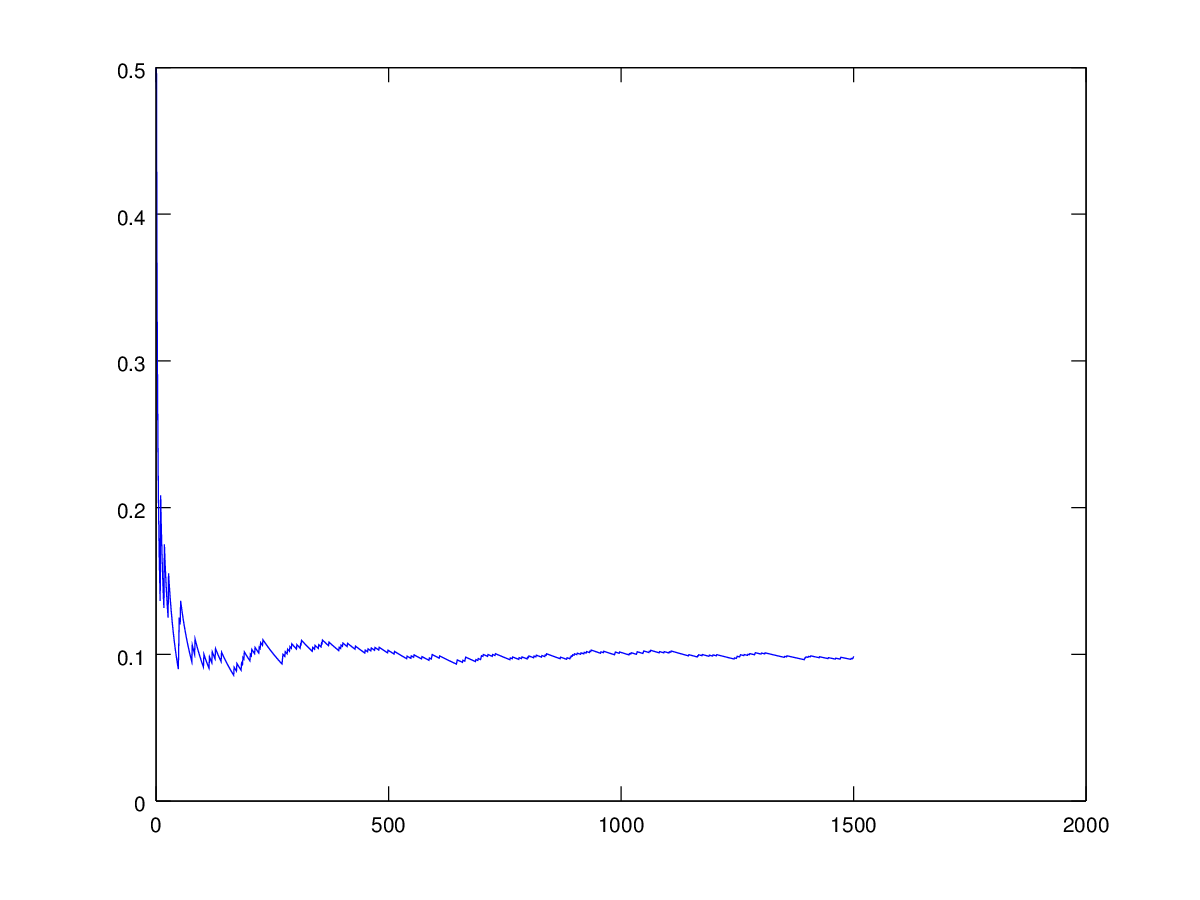
\includegraphics[width=0.7\textwidth]{poyla.png}
\caption{Urna de Poyla}
\label{Urna de Poyla}
\end{figure}


En esta gr\'afica se muestra la simulaci\'on de las urnas de Poyla. Como vimos en clase la proporci\'on de bolas rojas convergen, en esta gr\'afica se ilustra como la proporci\'on se tiende a estabilizar. Esto se debe al teorema de convergencia de martingalas ya que la martingala es positiva.

\end{ejercicio}

\begin{problema}[Ejercicios sueltos sobre martingalas]
\mbox{}\begin{enumerate}
\item Sea $\paren{X_n,n\geq 0}$ una sucesi\'on $\paren{\F_n}$-adaptada. Pruebe que\begin{esn}
\sum_{k=1}^n X_k-\espc{X_k}{\F_{k-1}}, \quad n\geq 0
\end{esn}es una $\paren{\F_n}$-martingala.

Demostraci\'on.

Denotemos a $M_n=\sum_{k=1}^n X_k-\espc{X_k}{\F_{k-1}}, \quad n\geq 0$.
\begin{enumerate}
\item Como $X_k$ es  $\F_k$-medible para todo $k\leq n$ entonces $X_k$ es $\F_n$-medible,ya que $X$ es $\F_n$-adaptada. Tambien sabemos por definici\'on de esperanza condicional que $\espc{X_k}{\F_{k-1}}$ es $\F_{k-1}$-medible, entonces $\espc{X_k}{\F_{k-1}}$ es $\F_n$-medible para todo $k\leq n$. Por lo tanto $M_n$ es $\F_n$-medible.
\item Por hip\'otesis $X_k\in L_1$ esto tambien nos indica que $\espc{X_k}{\F_{k-1}}\in L_1$, como $M_n$ es suma finita de variables aleatorias en $L_1$ entonces $M_n\in L_1$.

\item Propiedad de Martingala:
\begin{align}
\espc{M_n}{\F_{n-1}}&= \espc{\sum_{k=1}^n X_k-\espc{X_k}{\F_{k-1}}}{\F_{n-1}} \notag \\
&=\sum_{k=1}^n\espc{ X_k-\espc{X_k}{\F_{k-1}}}{\F_{n-1}} \notag \\
&=\sum_{k=1}^n\espc{ X_k}{\F_{n-1}}-\espc{\espc{X_k}{\F_{k-1}}}{\F_{n-1}} \notag
\intertext{Ya que $X_{k}$ es $\F_{n-1}$-medible para todo $k\leq n-1$}
&=\espc{ X_n}{\F_{n-1}}+\sum_{k=1}^{n-1} X_k-\sum_{k=1}^n\espc{\espc{X_k}{\F_{k-1}}}{\F_{n-1}} \notag
\intertext{Como $\espc{X_k}{\F_{k-1}}$ es $\F_{n-1}$-medible para toda $k\leq n$}
&=\espc{ X_n}{\F_{n-1}}+\sum_{k=1}^{n-1} X_k-\sum_{k=1}^n\espc{X_k}{\F_{k-1}} \notag \\
&=\sum_{k=1}^{n-1} X_k-\sum_{k=1}^{n-1}\espc{X_k}{\F_{k-1}} \notag \\
&=M_{n-1} \notag
\end{align}

Por lo tanto $M_n$ es martingala.
\end{enumerate}

\item{Descomposici\'on de Doob para submartingalas}: Sea Sea \(X=\paren{X_n}_{n\in\na}\) una submartingala. Pruebe que \(X\) se puede descomponer de manera \'unica como \(X=M+A\) donde \(M\) es una martingala y \(A\) es un proceso previsible con \(A_0=0\). Sugerencia: Asuma que ya tiene la descomposici\'on y calcule esperanza condicional de \(X_{n+1}\) dada \(X_n\). 

Como $X_n$ es submartingala podemos utilizar el inciso anterior para construir una martingala que dependa de $X_n$. A esa la denotaremos como $M_n=\sum_{k=1}^n X_k-\espc{X_k}{\F_{k-1}}+X_0$, al añadirle el $X_0$ sigue siendo martingala el proceso. Si suponemos que ya conocemos la descomposici\'on tenemos que:
\begin{esn}
X_n=M_n+A_n=\sum_{k=1}^n X_k-\espc{X_k}{\F_{k-1}}+X_0+A_n
\end{esn}
Despejando a $A_n$ tenemos que:
\begin{esn}
A_n=\sum_{k=1}^n \espc{X_k}{\F_{k-1}}-X_{k-1}
\end{esn}
Efectivamente $A_n$ es un proceso previsible ya que $\espc{X_k}{\F_{k-1}},X_{k-1}$ son $\F_{n-1}$-medibles.

Como $X_n$ es sub-martingala entonces $\espc{X_k}{\F_{k-1}\geq X_{k-1}}$. Por lo tanto $A_n$ es un proceso positivo. Por lo tanto las $A_n$ son crecientes.

La unicidad se da ya que si existen dos descomposiciones $M_n^1,A_n^1,M_n^2, A_n^2$ y si definimos $Y_n=M_n^1-M_n^2=A_n^1-A_n^2$. Por una parte tenemos que cumple la propiedad de Martingala y por otra parte cumple la propiedad de previsibilidad, es decir:
\begin{align}
\espc{Y_n}{\F_{n-1}}&=Y_{n-1} \notag \\
\espc{Y_n}{\F_{n-1}}&=Y_{n} \notag
\intertext{Si restamos las ecuaciones tenemos que:}
0&=Y_{n}-Y_{n-1} \notag \\
0&=A_{n}^{1}-A_{n-1}^{1}-(A_{n}^{2}-A_{n-1}^{2})\notag
\intertext{Como $A_{0}^{1}=0=A_{0}^{2}$ entonces tenemos que:}
0&=A_{1}^{1}-A_{1}^{2} \notag \\
A_{1}^{1}&=A_{1}^{2} \notag
\intertext{Recursivamente $A_{n}^{1}=A_{n}^{2}$ $\Rightarrow$ $Y=0$:}
M_{n}^{1}&=M_{n}^{2} \notag
\end{align}

Por lo tanto la descomposici\'on es \'unica.
\item Sea \(S_n=\xi_1+\cdots+\xi_n\) donde las variables \(\xi\) son independientes y \(\xi_i\) tiene media cero y varianza finita \(\sigma_i^2\). Pruebe que si \(\sum_i \sigma_i^2<\infty\) entonces \(S_n\) converge casi seguramente y en \(L_2\) conforme \(n\to\infty\). Construya un ejemplo de variables aleatorias \(\xi_i\) tales que la serie \(\sum_i \xi_i\) sea casi seguramente absolutamente divergente y casi seguramente condicionalmente convergente (considere ejemplos simples!). Explique heur\'isticamente por qu\'e cree que suceda esto.
%Ser\'a que \sum_i\abs{x_i}=\infty casi seguramente si \sum_i\abs\esp{\xi_i}=\infty? 

Sea $\F_n=\sag{\xi_1,\ldots,\xi_n}$. Hemos visto anteriormente que $\paren{X_n}_{n=1}^\infty$ es una martingala respecto a $\paren{\F_n}_{n=1}^\infty$. Adem\'as por la desigualdad de Cauchy-Schwartz, sabemos que\begin{esn}
\esp{\abs{X_n}}\leq \paren{\esp{X_n^2}}^{1/2}=\esp{\paren{\sum_{i=1}^n\xi_i}^2}^{1/2}
\end{esn}y como las variables aleatorias $\paren{\xi_i}_{i-1}^\infty$ son independientes y tienen media cero, su segundo momento es igual a su varianza  y la varianza de la suma (que corresponde tambi\'en  a su segundo momento) es igual a la suma de las varianzas, por lo que\begin{esn}
\esp{\abs{X_n}}\leq \paren{\sum_{i=1}^n\var{\xi_i}}^{1/2}\leq \paren{\sum_{i=1}^\infty\var{\xi_i}}^{1/2}<\infty,
\end{esn}por lo que la martingala $\paren{X_i}_{i=1}^\infty$ satisface las condiciones del teorema de convergencia casi segura de martingalas y por lo tanto, converge casi seguramente a una variable aleatoria que pertenece a $ L_1$.

El ejemplo es el siguiente:

Sea $\xi_i$ una variable aleatoria que toma los valores -1 y 1 con probabilidad $1/2$ Definimos la serie
$X_n=\sum_{i=1}^n \xi_i /i$, esta serie es casi seguramente absolutamente divergente debido a que.
\begin{esn}
\sum_{i=1}^{\infty} \abs{\xi_i}/i=\sum_{i=1}^{\infty} 1 /i=\infty .
\end{esn}



\item Sean \(X\) y \(Y\) dos martingalas (respecto de la misma filtraci\'on) y tales que \(\esp{X_i},\esp{Y_i}<\infty\) para toda \(i\). Pruebe la siguiente f\'ormula de integraci\'on por partes: $$ \esp{X_nY_n}-\esp{X_0Y_0}=\sum_{i=1}^n \esp{\paren{X_i-X_{i-1}}\paren{Y_i-Y_{i-1}}} . $$

Demostraci\'on

\begin{align}
\sum_{i=1}^n \esp{\paren{X_i-X_{i-1}}\paren{Y_i-Y_{i-1}}}&= \sum_{i=1}^n \esp{X_iY_i-X_{i-1}Y_i-X_iY_{i-1}+X_{i-1}Y_{i-1}} \notag \\
&=\sum_{i=1}^n \esp{X_iY_i}-\esp{X_{i-1}Y_i}-\esp{X_iY_{i-1}}+\esp{X_{i-1}Y_{i-1}} \notag \\
&=\sum_{i=1}^n \esp{X_iY_i}-\esp{\espc{X_{i-1}Y_i}{\F_{i-1}}} \notag \\
&-\esp{\espc{X_iY_{i-1}}{\F_{i-1}}}+\esp{X_{i-1}Y_{i-1}} \notag 
\intertext{Como $X_{i-1},Y_{i-1}$ son $F_{i-1}$-medibles:}
&=\sum_{i=1}^n \esp{X_iY_i}-\esp{X_{i-1}\espc{Y_i}{\F_{i-1}}} \notag \\
&-\esp{Y_{i-1}\espc{X_i}{\F_{i-1}}}+\esp{X_{i-1}Y_{i-1}} \notag 
\intertext{Como $X_i,Y_i$ son martingalas:}
&=\sum_{i=1}^n \esp{X_iY_i}-\esp{X_{i-1}Y_{i-1}} \notag \\
&-\esp{Y_{i-1}X_{i-1}}+\esp{X_{i-1}Y_{i-1}} \notag \\
&=\sum_{i=1}^n \esp{X_iY_i}-\esp{X_{i-1}Y_{i-1}} \notag \\
&=\esp{X_nY_n}-\esp{X_{0}Y_{0}}.
\end{align}

\item{Desigualdad de Azema-Hoeffding}
        \begin{enumerate}
        \item Muestre que si \(Y\) es una variable aleatoria con valores en \([-c,c]\) y media cero entonces, para \(\theta\in\re\)
                        $$\esp{e^{\theta Y}}\leq\imf{\cosh}{\theta c}\leq \imf{\exp}{\frac{1}{2}\theta^2c^2}. $$
                        
                        Como $e^{\theta y}$ es una funci\'on convexa tenemos que:
                        \begin{esn}
                        e^{\theta y}\leq \frac{c-y}{2c}e^{-\theta c}+\frac{c+y}{2c}e^{\theta c}=\frac{e^{\theta c}+e^{-\theta c}}{2}+y(\frac{e^{\theta c}-e^{-\theta c}}{2c})
                        \end{esn}
                        Calculando la esperanza de ambos lados de la desiguañdad obtenemos que:
                        \begin{esn}
                        \esp{e^{\theta Y}}\leq \esp{\frac{e^{\theta c}+e^{-\theta c}}{2}+Y(\frac{e^{\theta c}-e^{-\theta c}}{2c})}
                        \end{esn}
                        Como la $\esp{Y}=0$, se sigue el resultado $\esp{e^{\theta Y}}\leq cosh\paren{\teta c}$.
                        
                        Para la segunda parte de la desigualdad, nos fijamos en la expansion de Taylor de $\cosh\paren{\theta c}$:
                        \begin{align}
                      \cosh\paren{\theta c}&=\sum_{k=1}^\infty \frac{\paren{\theta c}^{2k}}{2k!} \notag \\
                      &\leq \sum_{k=1}^\infty \frac{\paren{\theta c}^{2k}}{2^k\paren{k!}} \notag \\
                      &=e^{\frac{\theta^2c^2}{2}}.\notag
                        \end{align} 
                        
        \item Pruebe que si \(M\) es una martingala nula en cero tal que para algunas constantes \(\paren{c_n,n\in\na}\) se tiene que
                        $$\abs{M_n-M_{n-1}}\leq c_n\quad\forall n $$
                        entonces, para \(x>0\)
                        $$
                        \proba{\max_{k\leq n} M_k\geq x}\leq \imf{\exp}{\frac{x^2}{2\sum_{k=1}^n c_k^2}}.
                        $$
                        En esta parte utilizaremos una  desigualdad de Doob que viene en las notas y dice que para una sub-martingala $M_n$ se tiene:
                        			\begin{esn} 
                        			\lambda\p\paren{\max_{1\leq i \leq n}M_i^+>\lambda} \leq \esp{M_n^+}
                        			\end{esn}
                        			En nuestro caso $M_n$ es martingala por lo que $e^{\theta M_n}$ es una sub-martingala positiva, aplicando la desigualdad de la proposici\'on anterior a esta sub-martingala  y tomando $\lambda = e^{\theta x}$ obtenemos que:
                        			\begin{esn}
                        			 e^{\theta x}\proba{\max_{1\leq i \leq n} e^{\theta M_i}> e^{ \theta x}} \leq \esp{ e^{\theta M_n}}
                        			\end{esn}
                        			Como $\set{\max_{1\leq i \leq n} e^{\theta M_i}> e^{\theta x}}=\set{\max_{1\leq i \leq n}  M_i>  x}$, entonces:
                        			\begin{esn}
                        			\proba{\max_{1\leq i \leq n}  M_i>  x} \leq  e^{-\theta x} \esp{ e^{\theta M_n}}
                        			\end{esn}
                        			Acotando a la martingala $M_n$ la cual es nula en $0$:
                        			\begin{align}
                        			\abs{M_n}&=\abs{\sum_{i=1}^{n}M_i-M_{i-1}}\notag \\
                        			&\leq \sum_{i=0}^{n}\abs{M_i-M_{i-1}}\notag \\
                        			&\leq\sum_{i=0}^{n}c_i=c^* \notag
                        			\end{align}
                        			Entonces $\abs{M_n}$ es acotada por $c^*$ por lo que podemos aplicar la desigualdad del ejercicio anterior
                        			\begin{esn}
                        			 \esp{ e^{\theta M_n}} \leq e^{\frac{1}{2}\theta^2(c^*)^2}
                        			\end{esn}
                        			Por lo tanto $\p\paren{\max_{1\leq i \leq n}  M_i>  x} \leq  e^{-\theta x} e^{\frac{1}{2}\theta^2(c^*)^2}$.Tomando a $\theta=\frac{x}{(c^*)^2}>0$, entonces
                        			\begin{align}
                        			\p\paren{\max_{1\leq i \leq n}  M_i>  x} &\leq exp\paren{-\frac{1}{2}\frac{x^2}{(c^*)^2}} \notag \\  &=exp\paren{\frac{-x^2}{2\paren{\sum_{i=1}^{n}c_i}^2}}\notag \\
                        			\end{align}
        \end{enumerate}
\end{enumerate}
\end{problema}
\begin{problema}
Sea $S_n=\sum_{i=1}^n X_i$ donde $X_1,X_2,\ldots$ son iid. Sea\begin{esn}
\imf{\phi}{\lambda}=\esp{e^{\lambda S_n}}\in (0,\infty].
\end{esn}
\begin{enumerate}
\item Pruebe que si existen $\lambda_1<0<\lambda_2$ tales que $\imf{\phi}{\lambda_i}<\infty$ entonces $\imf{\phi}{\lambda}<\infty$ para toda $\lambda\in [\lambda_1,\lambda_2]$. Sugerencia: escriba $\lambda=a\lambda_1+(1-a)\lambda_2$ para alg\'un $a\in [0,1]$ y aplique la desigualdad de H\"older. A partir de ahora se asume la premisa de este inciso.

Sea $\lambda\in [\lambda_1,\lambda_2]$ entonces $\exists$ $a\in [0,1]$ $\lambda=a\lambda_1+(1-a)\lambda_2$.

\begin{align}
\imf{\phi}{\lambda}&=\esp{e^{\lambda S_n}} \notag \\
&= \esp{e^{\paren{a\lambda_1+(1-a)\lambda_2} S_n}} \notag \\
&= \esp{e^{\paren{a\lambda_1}S_n}e^{(1-a)\lambda_2 S_n}} \notag
\intertext{Aplicando la desigualdad de Holder:}
&\leq \esp{e^{\paren{\lambda_1}S_n}}^a\esp{e^{\lambda_2 S_n}}^{1-a} \notag
\end{align}

Como la $\esp{e^{\paren{\lambda_1}S_n}}^a,\esp{e^{\lambda_2 S_n}}^{1-a}<\infty$ tenemos que $\imf{\phi}{\lambda}<\infty$ para toda $\lambda \in [\lambda_1,\lambda_2]$.

\item Pruebe que $\esp{\abs{S_n}^k}<\infty$ para toda $k\geq 0$. 

Sea $\lambda \in [\lambda_1,\lambda_2]$, definimos $X_m=\sum_{k=0}^{m}\frac{\abs{\lambda S_n}^k}{k!}$. Expresando como serie de taylor a $e^{\abs{\lambda S_n}}$ tenemos que:
\begin{align} 
\esp{e^{\abs{\lambda S_n}}}&=\esp{\lim_{m \rightarrow \infty}\sum_{k=0}^{m}\frac{\abs{\lambda S_n}^k}{k!}}\notag \\
&=\esp{\lim X_m}
\intertext{Como $X_m$ es una sucesi\'on creciente, ya que los terminos de la suma son positivos, se tiene  por el teorema de la convergencia mon\'otona que:}
&=\lim_{m \rightarrow \infty}\esp{X_m}\notag\\
&=\sum_{k=0}^{\infty}\frac{\abs{\lambda}^k \esp{\abs{S_n}^k}}{k!}\notag 
\end{align} 


Entonces:
\begin{align}
\esp{e^{\abs{\lambda S_n}}}&=\esp{e^{\lambda S_n}\indi{\lambda S_n \geq 0}}+\esp{e^{-\lambda S_n}\indi{\set{\lambda S_n <0}}} \notag \\
&\leq \esp{e^{\lambda S_n}}+\esp{e^{-\lambda S_n}} \notag
\intertext{Por inciso anterior tenemos que:}
&=\phi(\lambda)+\phi(-\lambda) < \infty. \notag
\end{align}


Por lo tanto $\sum_{k=0}^{\infty}\frac{\abs{\lambda}^k \esp{\abs{S_n}^k}}{k!}\ < \infty$.

Por lo tanto $\esp{\abs{S_n}^k} < \infty$ para toda $k\in \na$.

\item Sea $M^\lambda_t=e^{\lambda S_t}/\imf{\phi}{\lambda}$. Argumente que si $M^n$ es el proceso dado por\begin{esn}
M^n_t=\left.\frac{\partial^n}{\partial \lambda^n}\right|_{\lambda=0}M^\lambda_t,
\end{esn}entonces $M^n$ es una martingala para toda $n$. 
\item Calcule las primeras $4$ martingalas resultantes si $\proba{X_i=\pm 1}=1/2$. Util\'icelas para calcular el valor de $\esp{T^2}$ donde\begin{esn}
T=\min\set{n\geq 0: S_n\in\set{-a,b}}
\end{esn}y $a,b>0$. 
\end{enumerate}

\defin{Categor\'ias:} Caminatas aleatorias, muestreo opcional, ejemplos de martingalas. 
\end{problema}

\begin{problema}
Sea $M$ una $\paren{\F_n}$-martingala. Pruebe que si $T$ es un tiempo de paro finito entonces $\esp{M_T}=\esp{M_0}$ bajo cada una de las siguientes condiciones:
\begin{enumerate}
\item $M$ es acotada.

Si $M$ es acotada entonces $\abs{M_n}\leq K$ para toda $n\in\na$ esto implica que $M_{T\wedge n}$ tambien es acotada. Adem\'as como $T\wedge n$ es un tiempo de paro acotado por el teorema de muestreo opcional de Doob entonces $\esp{M_{T\wedge n}}=\esp{M_0}$. Ya que $M_{T\wedge n}$ converge a $M_T$, aplicande el teorema de convergencia acotada tenemos que $\esp{M_{T\wedge n}}$ converge a $\esp{M_{T}}$ pero la esperanza de $\esp{M_{T\wedge n}}=\esp{M_{0}}$ para toda $n\in \na$. Por lo tanto $\esp{M_T}=\esp{M_0}$.


\item $T$ es integrable y la sucesi\'on $\paren{M_n-M_{n-1}}$ es acotada.

Como la sucesi\'on $\paren{M_n-M_{n-1}}$ es acotada entonces $\abs{\paren{M_n-M_{n-1}}}\leq K$.
\begin{esn}
\abs{\paren{M_{T\wedge n}-M_{0}}}=\abs{\sum_{i=1}^{T\wedge n}\paren{M_i-M_{i-1}}}\leq\sum_{i=1}^{T\wedge n}\abs{\paren{M_i-M_{i-1}}}\leq T K.
\end{esn}

Entonces la sucesi\'on $M_{T\wedge n}-M_{0}$ dominada por $KT$. Utilizando el teorema de muestreo opcinal de Doob sabemos que $\esp{M_{T\wedge n}-M_{0}}=0$ para toda $n\in \na$. Podemos utiliar el teorema e convergencia dominada ya que $KT$ es integrable entonces $\esp{M_T-M_0}=0$. Por lo tanto $\esp{M_T}=\esp{M_0}$.
\item $\paren{M_{n\wedge T}}$ es uniformemente integrable.

Sabemos que $\M_{n\wedge T}$ converge a $M_T$,  ademas como $M_{n\wedge T}$ es uniformemente integrable sabemos que $M_{T}$ es integrable y $\esp{M_{n\wedge T}}$ converge a $\esp{M_{T}}$. Pero por el teorema de muestreo opcional de Doob como $T\wedge n$ es un tiempo de paro acotado la $\esp{M_{T\wedge n}}=\esp{M_0}$. Por lo tanto $\esp{M_{T}}=\esp{M_0}$.

\end{enumerate}

\defin{Categor\'ias: } Muestreo opcional. 
\end{problema}

\begin{problema}
Sea $M$ una $\paren{\F_n}$-martingala con saltos acotados. Sean
\begin{esn}
C=\set{\limsup M_n=\liminf M_n\in\re}\quad\text{y}.
\end{esn}
Pruebe que $\proba{C\cup D}=1$. Deduzca que las caminatas aleatorias centradas con saltos acotados oscilan. Sugerencia: Para cada $K>0$ defina\begin{esn}
T=\min\set{n\geq 0: \abs{M_n}\geq K}
\end{esn}y aplique el teorema de convergencia de martingalas a $M^T$. 

Sea $M$ una caminata aleatoria no trivial con saltos integrables en $-1,0,1,\ldots$ y  media cero. Pruebe que $\proba{M\text{ converge en }\na}=0$ y  concluya que $\liminf M_n=-\infty$ casi seguramente. (Este resultado permitir\'a dar una prueba adicional de que un Galton-Watson cr\'itico se extingue).  Sugerencia: proceda como en el p\'arrafo anterior y pruebe la integrabilidad uniforme de $M_{T\wedge n},n\in\na$.

\defin{Categor\'ias: } Teoremas de convergencia de martingalas
\end{problema}

\begin{problema}
Sean $X_1,X_2,\ldots$ variables aleatorias intercambiables:\begin{esn}
\paren{X_1,\ldots, X_n}\stackrel{d}{=}\paren{X_{\pi_1},\ldots, X_{\pi_n}}
\end{esn}para cada permutaci\'on $\sigma$ de $\set{1,\ldots,n}$. 
\begin{enumerate}
\item Para $\G,\h$ sub$\sigma$-\'algebras de $\F$ definimos a $\G\vee\h=\sag{\G\cup\h}$. Sea \begin{esn}
\G^n=\sag{\imf{f}{X_1,\ldots, X_n}: \fun{f}{\re^n}{\re}\text{ es sim\'etrica}}\vee\sag{X_{n+1},X_{n+2},\ldots}. 
\end{esn}Pruebe que $\G^n,n\geq 1$ es una filtraci\'on al rev\'es. Sea $\G$ su intersecci\'on.
\item Para cada $A\in\mc{B}_{\re}$, defina a\begin{esn}
\imf{\Xi_n}{A}=\frac{1}{n}\sum_{i=1}^n \indi{X_i\in A}.
\end{esn}Pruebe que\begin{esn}
\probac{X_1\in A}{\G^n}=\imf{\Xi_n}{A}. 
\end{esn}?`Por qu\'e puede definir a  $\imf{\Xi}{A}=\lim_{n\to\infty}\imf{\Xi_n}{A}$?
\item Al considerar a la martingala\begin{esn}
\frac{1}{n\paren{n-1}}\sum_{1\leq i<j\leq n}\indi{X_i\in A}\indi{X_j\in A},
\end{esn}pruebe que $\probac{X_1\in A,X_2\in A}{\G}=\probac{X_1\in A}{\G}\probac{X_2\in A}{\G}$. Extienda la afirmaci\'on de independencia condicional anterior a $X_1,\ldots, X_n$. 
\end{enumerate}

\defin{Cagegor\'ias: }Teorema de convergencia de martingalas, teorema de de Finetti.
\end{problema}

\begin{ejercicio}
\mbox{}
\begin{enumerate}
\item Ejecute y explique la funci\'on del siguiente c\'odigo en Octave. Comente qu\'e teoremas del curso (y del curso de probabilidad) son importantes para interpretar la figura.

\item Ejecute y explique la funci\'on del siguiente c\'odigo en Octave. Incluya una gr\'afica en la que la longitud de la variable k sea mayor a 1000. (Puede modificar el programa...) En la gr\'afica observara un esbozo de la trayectoria de un proceso de ramificaci\'on continuo (en una escala distinta...).


\end{enumerate}
\end{ejercicio}

%
%\begin{problema}
%Sean $\F_1,\F_2,\ldots $ y $\G$ sub\sa s de $\F$. Decimos que $\F_1,\F_2,\ldots$ son condicionalmente independientes dada $\G$ si para cualquier $H_i$ que sea $\F_i$ medible y acotada se tiene que\begin{esn}
%\espc{H_1\cdots H_n}{\G}=\espc{H_1}{\G}\cdots \espc{H_n}{\G}.
%\end{esn}
%\begin{enumerate}
%\item ?`Qu\'e quiere decir la independencia condicional cuando $\G=\set{\oo,\emptyset}$?
%\item Pruebe que $F_1$ y $\F_2$ son condicionalmente independientes dada $\G$ (denotado $\condind{\F_1}{\F_2}{\G}$) si y s\'olo si para cualquier $H$ que sea $\F_1$-medible y acotada se tiene que\begin{esn}
%\espc{H}{\F_2,\G}=\espc{H}{\G}.
%\end{esn}
%\item Pruebe que $\F_1,\F_2,\ldots, $ son condicionalmente independientes dada $\G$ si y s\'olo si para cada $n\geq 1$, $\F_{n+1}$ es condicionalmente independiente de $\F_1,\ldots, \F_n$ dada $\G$. 
%\end{enumerate}
%
%\defin{Categor\'ias: } Esperanza condicional, Independencia condicional.
%\end{problema}
%
%\begin{problema}
%Sea $\mu$ una distribuci\'on de progenie y defina $\tilde \mu_j=\mu_{j+1}$. Sea $S=\paren{S_n}$ una caminata aleatoria con distribuci\'on de salto $\tilde\mu$. Sea $k$ un entero no-negativo y defina recursivamente\begin{esn}
%Z_0=k=C_0,\quad Z_{n+1}=k+S_{C_n}\quad\text{y} C_{n+1}=C_n+Z_{n+1}.
%\end{esn}
%\begin{enumerate}
%\item Pruebe que $Z_n\geq 0$ para toda $n$ y que si $Z_n=0$ entonces $Z_{n+1}=0$.
%\item Pruebe que $C_n$ es un tiempo de paro para la filtraci\'on can\'onica asociada a $S$.
%\item Pruebe que $Z$ es un proceso de Galton-Watson con ley de progenie $\mu$. 
%\item Pruebe que si $S$ alcanza $-1$ entonces existe $n$ tal que $Z_n=0$. Deduzca que si la media de $\mu$ es $1$ entonces $Z$ se extingue. (Sugerencia: utilice un ejercicio anterior sobre martingalas con saltos acotados hacia abajo.) 
%\end{enumerate}
%
%\defin{Categor\'ias: } Caminatas aleatorias, Procesos de Galton-Watson%, Propiedad de Markov fuerte.
%\end{problema}
%
%\begin{problema}
%Sea $\mu$ una distribuci\'on de progenie y defina $\tilde \mu_j=\mu_{j+1}$. Sea $\nu$ una distribuci\'on en $\na$. Consideremos a dos caminatas aleatorias $S=\paren{S_n}$  y $T$ con  distribuci\'ones de salto $\tilde\mu$ y $\nu$.
%\begin{enumerate}
%\item ?`Qu\'e significa que $S$ y $T$ sean independientes? As\'umalo.
%\item Sea $k$ un entero no-negativo y defina recursivamente\begin{esn}
%Z_0=k=C_0,\quad Z_{n+1}=k+S_{C_n}+T_n\quad\text{y} C_{n+1}=C_n+Z_{n+1}.
%\end{esn}
%\item Pruebe que $Z_n\geq 0$ para toda $n$.
%\item Pruebe que $C_n=k\in\F^S_k\cap\F^T_n$.
%\item Pruebe que $Z$ es un proceso de Galton-Watson con inmigraci\'on.
%\end{enumerate}
%
%\defin{Categor\'ias: } Caminatas aleatorias, Procesos de Galton-Watson, Construcci\'on de procesos estoc\'asticos
%\end{problema}
%
%\begin{problema} %Construcci\'on tipo Poisson 
%Sean $\mu$ y $\nu$ una distribuci\'on de progenie y de inmigraci\'on. Sean $Y_1,Y_2,\ldots$ independientes y de ley $\nu$. Suponga que condicionalmente a $Y$, $X^0,X^1,X^2,\ldots$ son procesos de Galton-Watson independientes tales que $X^0_0=k$ y $X^k_0=Y_k$ para $k\geq 1$. Pruebe que si\begin{esn}
%Z_n=\sum_{k=0}^n X^k_{n-k},
%\end{esn}entonces $Z$ es un proceso de Galton-Watson con distribuciones de progenie e inmigraci\'on $\mu$ y $\nu$ que comienza en $k$. 
%
%\defin{Categor\'ias: } Procesos de ramificaci\'on
%\end{problema}
%
%\begin{problema}
%Para cada par de medidas de probabilidad en $\na^\na$ $\p_1$ y $\p_2$ definimos a la convoluci\'on de $\p_1$ y $\p_2$, denotada $\p_1 *\p_2$, como la distribuci\'on de $\paren{S^1_k+S^2_k,k\geq 0}$ donde $S^1$ y $S^2$ son independientes y de distribuciones $\p_1$ y $\p_2$ respectivamente.
%\begin{enumerate}
%\item ?` Cu\'al es la relaci\'on entre las distribuciones finito-dimensionales de $\p_1$, $\p_2$ y $\p_1*\p_2$?
%\item Sea $\p_k^\mu$ la distribuci\'on de un proceso de Galton-Watson  de ley de reproducci\'on $\mu$ que comienza en $k$. Pruebe que $\p_{k_1}*\p_{k_2}=\p_{k_1+k_2}$.
%%\item Caracterizaci\'on de leyes markovianas con la propiedad de ramificaci\'on.
%\end{enumerate}
%
%\defin{Categor\'ias: } Distribuciones finito-dimensionales, Procesos de ramificaci\'on.
%\end{problema}
\bibliographystyle{amsalpha}
\end{document}